In this chapter, we will analyze the literature and background: we will first examine the more general field of Human-Computer Interaction (HCI), passing then to Human-Robot Interaction (HRI) and, finally, Human-Drone Interaction (HDI), what are the purposes, the achievement, and the limitations of this research. 
Next, we will move to the programming environments for both single and multiple drones, understanding 
which are the main design paradigms and solutions available. 


\section{Human-Robot Interaction}\label{sec:soa_hri}
We live in an era where humans and computers are increasingly in close contact. In the last 40 years, the continuous and exponential growth 
in computational power and storage capacity, but even more relevant, the huge spread of technologies in every aspect of our lives,
has moved the concept of Human-Computer interaction to a central stage of research. 
With the massive amount of new designs of technologies and systems, this relation grows exponentially in complexity, 
and the importance of profoundly understanding it is a key aspect of bringing innovation to the next step and, more importantly, 
avoiding the risk of incurring harmful and undesired situations.

Human-Computer Interaction (HCI) is a discipline concerned with the design, evaluation, and implementation of interactive computing systems for human use
and with the study of major phenomena surrounding them~\cite{sinha2010human}.
The role of this discipline is to understand in depth the relation between humans and computers, creating user interfaces and experiences that are effective, efficient, and enjoyable. 
On the other side, HCI must also understand the limits and the risks associated with those new interfaces, which should guide governments around the world to regulate 
and control the expansion of such technologies in a sane manner but avoid limiting their potentiality.

Regarding our work, it is better to narrow down the concept of HCI to a subfield of research: Human-Robot Interaction (HRI). 
Actually, HRI is not only a subfield of the more general HCI; instead, it is a multidisciplinary field with the influence of HCI, 
artificial intelligence, natural language understanding, and social science.
The primary goal of HRI is to define a general human model that could lead to principles and algorithms allowing more natural and 
effective interactions between humans and robots~\cite{hri2009davidMaya}.

\subsection{The Interaction Between Human and Robot}\label{subsec:the_interaction}
The Human is an extremely sophisticated biological system characterized by an impressive, complex, and powerful brain that is the main
coordinator and central actor in the whole human system. Given this complexity, for our purpose, we can model it using
the Model Human Processor (MPH) proposed by Card, Moran, and Newell in 1983~\cite{card1986model}. 

MPH describes the Human as composed of 3 subsystems: the perceptual, motor, and cognitive systems. 
Each of them has a processor and memory.
Input in humans occurs mainly through the senses and output through the motor controls of the effectors~\cite{dix2010human}. 
Therefore, vision, hearing, and touch are the most important senses in HRI, while fingers, voice, eyes, 
head and body position are the primary effectors.

On the other hand, the computer is a straightforward machine that processes the input data that it receives into outputs. 
The processor is the leading actor in the data transformation process: it can perform arithmetic and logic operations very fast. 
Both input and output data for the computer are encoded binary sequences.

The interaction, with or without a robot, is a process of information transfer between two (or multiple) systems. 
The outputs of one system are the inputs of the other and vice versa. 
In the interaction, it is immediately evident that the human outputs are incompatible with the robot's input. 
Also, the outputs of a robot are not easily interpretable by a human. 
This profound discrepancy between the two is the domain of study for HRI; the user outputs need to be translated from body movements and voice to binary sequences, and, on the other hand, the robot outputs need to be translated from binary data to images, text, and sounds.

Initially, with computers becoming accessible to the public fifty years ago, command-line interaction was the only option for interacting with a computer. 
Today, interfaces have evolved into sophisticated forms such as advanced GUI, touchscreens, Augmented Reality, Virtual Reality, and Haptic interfaces. 
All these new interfaces make one side easier the lives of humans, but on the other side, they have inevitably brought values 
and ethics in technology design to the forefront of public debate: questions about the goals and politics of human-designed devices, 
and whether the social interactions of those devices are good, just, or fair~\cite{shilton2018hciEthics}. 

\subsection{HRI Taxonomy}\label{subsec:hri_taxonomy}
HRI is a highly heterogeneous field, and understanding the details of interactions between humans and robots is crucial for advancing this dynamic field. 
To define and better identify the diverse range of interactions between humans and robots, 
it is important to organize and classify the interactions in a structured taxonomy~\cite{yanco2004taxonomy}.

Following this taxonomy, HRI can be classified using the following attributes:

{\bfseries \scshape Task Type}:\\*
It is a high-level description of the task to be accomplished. It sets the tone for the system's design and use. 
Moreover, it implicitly represents the robot's environment. 
For example, the task classification could be \textit{urban search and rescue}, \textit{walking aid for blind people}, or \textit{hospital delivery robot}.

{\bfseries \scshape Task Criticality}:\\*
It measures the importance of getting the task done correctly in terms of its negative effects should problems occur. 
To mitigate the subjective nature of this attribute, it can take three values: \textit{high}, \textit{medium}, and \textit{low}.
The criticality classification could be \textit{high} for the urban search and rescue, \textit{medium} for the hospital delivery robot, and \textit{low} for a jogging companion robot.

{\bfseries \scshape Robot Morphology}:\\*
It can assume three values: \textit{anthropomorphic} (having a human-like appearance), \textit{zoomorphic} (having an animal-like appearance), 
and \textit{functional} (having an appearance that is neither human-like nor animal-like but is related to the robot's function).
It is an essential measure since people react differently based on their appearance.
Examples of this classification are shown in Figure~\ref{fig:robot_morphology}

{\bfseries \scshape Interaction Roles}:\\*
When humans interact with a robot, they can act in 5 different roles: \textit{supervisor} (monitor the behavior of a robot), 
\textit{operator} (control and modify the behavior of the robot), \textit{teammate} (work in cooperation together to accomplish a task), 
\textit{mechanic/programmer} (physically change the robot's hardware or software), and \textit{bystander} 
(needs to understand the robot's behavior to be in the same space).
For example, a firefighter who uses a drone for urban search and rescue assumes the role of \textit{operator} because they need to guide it to the rescue area. 
In the hospital delivery robot, the people in the hospital have the role of \textit{bystander}; they need to understand the drone behavior since they share the same space.
\\\\ % REASON FORMAT 
{\bfseries \scshape Type of Human-Robot Physical Proximity}:\\*
When interacting with the robot, a human can act at different levels of physical proximity: \textit{none} (the robot and the human are in different places), 
\textit{avoiding} (the robot is aware and avoids the user when approaching), \textit{passing} (the robot is not aware of the user, so the user needs to pass by), 
\textit{following} (the robot is aware and follows the user when approaching), 
\textit{approaching} (the robot and the user operate close without contact), and \textit{touching} (the robot and the user operate close with contact).

{\bfseries \scshape Decision Support for the Human}:\\*
It represents the type of information that is provided to operators for decision support. 
This taxonomy category has four subcategories: 
\begin{itemize}
    \item \textit{Available sensor information}: the full list of sensors available on the robot, e.g., an urban search and rescue robot could have: \textit{sonar}, \textit{LIDAR}, \textit{camera}
    \item \textit{Sensor information provided}: the partial list of sensors useful for decision support, e.g., the robot may use its sonar and LIDAR to navigate, but only a video image is provided in the interface.
    \item \textit{Type of sensor fusion}: is specified as a list of functions that combines multiple sensors available, e.g., if sonar and LIDAR values were used to build a map that was displayed, the sensor fusion list would contain \( {{sonar, lidar} \square map } \).
    \item \textit{Pre-processing}: is a list of functions that preprocess the values of the sensors before displaying them in the interface, e.g., if a video stream is processed before display to highlight regions of a particular color, say red, the list would include \( {video \square highlight red regions } \).
\end{itemize}

{\bfseries \scshape Time and Space}:\\*
Divides Human-Robot interaction into four categories based on whether the humans and robots interact at the same time (\textit{synchronous}) or different times (\textit{asynchronous}) and while in the same place (\textit{collocated}) or different places (\textit{non-collocated}).
The urban search and rescue robot is an example of \textit{synchronous} and \textit{collocated} time and space. 
In contrast, a space rover like Curiosity~\cite{curiosity} is definitely an example of \textit{asynchronous} and \textit{non-collocated}.

{\bfseries \scshape Autonomy Level and Amount of Intervention}:\\*
The autonomy level measures the percentage of time that the robot is carrying out its task on its own; 
the amount of intervention required measures the percentage of time that a human operator must be controlling the robot.

\begin{figure}[tb]
    \centering
    \subfloat[Anthropomorphic robot\label{fig:anthropomorphic_robot}]{
        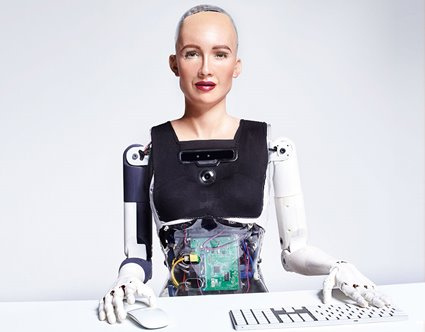
\includegraphics[width=0.28\textwidth]{soa/anthropomorphic}
    }
    \quad
    \subfloat[Zoomorphic robot\label{fig:zoomorphic_robot}]{
        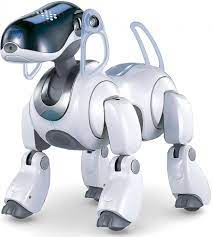
\includegraphics[width=0.28\textwidth]{soa/zoomorphic}
    }
    \quad
    \subfloat[Functional robot\label{fig:functional_robot}]{
        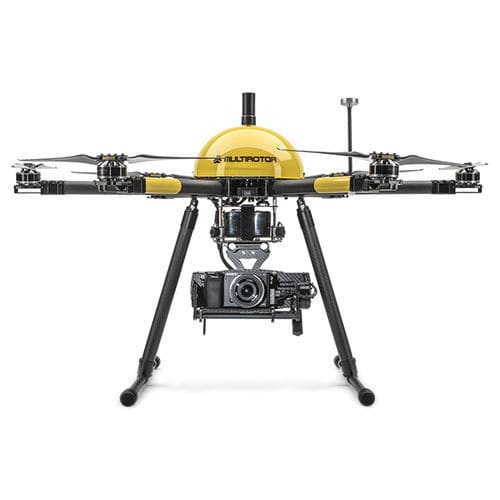
\includegraphics[width=0.28\textwidth]{soa/functional}
    }
    \caption{Robot morphology examples.}\label{fig:robot_morphology}
\end{figure}

In Table~\ref{table:taxonomy_target} we present the type of interaction that we are targeting in this thesis work using the taxonomy described above.

\begin{table}[tb]
\centering
    \begin{tabular}{|p{0.33\textwidth}|m{0.61\textwidth}|}
    \hline
    \rowcolor{bluepoli!40}
    \textbf{Attribute} & \textbf{Values} \\
    \hline \hline
    {\scshape Task Type} & Arbitrary interaction with nano drones in a small indoor environment to investigate Human-Drone relation \\
    \hline
    {\scshape Task Criticality} & Low \\
    \hline
    {\scshape Robot Morphology} & Functional \\
    \hline
    {\scshape Interaction Roles} & Mechanic/Programmer or Operator \\
    \hline
    {\scshape Physical Proximity} &  Any value \\
    \hline
    {\scshape Decision Support} & Available sensors: [proximity (x, y, z), localization (x, y, z), flow (vx, vy), video] \\
    \hline
    {\scshape Time and Space} & Synchronous and Collocated \\
    \hline
    {\scshape Autonomy Level} & Any value \\
    \hline
    {\scshape Amount of Intervention} & Any value \\
    \hline
    \end{tabular}
    \\[10pt]
    \caption[Taxonomy for interaction of target applications]{Categorization of interaction for target applications in our thesis work following the taxonomy proposed by Yanco and Drury~\cite{yanco2004taxonomy}.}\label{table:taxonomy_target}
\end{table}


\section{Human-Drone Interaction}\label{sec:soa_hdi}
Drones, also known as unmanned aerial vehicles (UAVs), are robots capable of flying autonomously or through different control modalities.
Until the early 2000s, drones were complex systems commonly seen in the military world and out of reach for civilians. 
Modern advancements in hardware and software technologies allow the development of smaller, easier-to-control, and lower-cost systems.
Drones are now found performing a broad range of civilian activities, and their usage is expected to keep increasing in the near future.
As drone usage increases, humans will interact with such systems more often; therefore, achieving a natural human-drone interaction is crucial.

Human-Drone Interaction (HDI) can be defined as the study field focused on understanding, designing, and evaluating drone systems 
for use by or with human users~\cite{tezza2019hdi}. Although some knowledge can be derived from the field of HRI, 
drones can fly in 3D space, which essentially changes how humans interact with them, making HDI a field of its own.
This field is relatively new in the research community, but in the last few years, the number of publications about HDI has grown exponentially.

\subsection{The Role of the Human During the Interaction}\label{subsec:hdi_interacction_role}
One of the core topics in the field of HDI is the role of humans during interaction with drones.
Depending on the drone's application and its level of autonomy, humans can play different roles when interacting with drone systems.

When the user pilots the drone to accomplish a given task by directly controlling the drone through a control interface, 
the user is considered an \textit{active controller} of the interaction. In these settings, the user's role is crucial to complete the given task; the drone instead acts as a mere executor of instructions. 
Examples of this type of interaction are waypoint navigation~\cite{hoppe2019droneOS} or artistic exhibitions~\cite{eriksson2020ethicsInMovement}.

The user acts as a \textit{recipient} when they do not control the drone, but they benefit from interacting with it. 
An example of this type of interaction is represented by delivery drones used to deliver a package~\cite{singireddy2018primeAir,hoppe2019droneOS, wingDrones}.

Another type of interaction role is when the drone acts as a \textit{social companion} for the user. 
In this case, the user might or might not be able to control the drone movement, but it holds a social interaction with it.
An example of this type of interaction is represented by Joggobot~\cite{graether2012joggobot}, a drone used as a companion for jogging.

The last type of role the user can play when interacting with a drone is the role of \textit{supervisor}.
Autonomous drones require users to act as supervisors either to pre-program the drone behavior or to 
supervise the flight itself in case of emergency. In this case, examples can be crop monitoring~\cite{dantu2011karma} or aerial photogrammetry~\cite{nex2014uav3Dmapping}, 

\subsection{The Drone's Control Modality}\label{subsec:hdi_drone_control_mod}
Usually, drones expose a control interface that allows users to control their behavior and eventually complete some tasks in the application domain.
Each control interface impacts how the pilot interacts with the drone in various aspects, 
such as training period, accuracy, latency, and interaction distance.

As drones became available to the public, the major drone producers felt the need to change their control modality 
from the standard remote controller to a more natural and easy-to-use interface.
A wide variety of control interfaces are available on the market today, 
ranging from standard remote controllers to very complex and advanced Brain Controlled Drones~\cite{lafleur2013quadcopterBCI}.

Drone's control interfaces can be classified as follows~\cite{tezza2019hdi}:

\textbf{\textit{Remote Controller}} is the standard and most commonly used interface, where the user directly controls the drone movements.
This control modality provides low latency and precise control, but on the other hand, it is less intuitive and usable 
than natural user interfaces. The usability and easiness of this interface strongly depend on the drone's level of autonomy.

\textbf{\textit{Gesture-based interface}} is a control modality where the user pilots the drone with body movements.
Usually, the drone uses a camera or a Kinect device to extract spatial information and recognize postures. 
When users are asked to interact with a drone without any instruction, gesture interaction is the primary choice of most users, 
and this indicates that the training period of this interface is almost close to zero~\cite{cauchard2015droneAndMe}. 
Gesture-based controls have a high latency and lower control precision compared to other control modalities. 
The flight space for drones that use this control method is sensibly reduced since the pilot needs to be close to the drone during the flight.

\textbf{\textit{Speech-based interface}} is a control modality where the user pilots the drone using vocal commands. 
As for gesture-based, this interface is also a natural user interface with a low training period and high usability.
They also share the problems of user proximity and high latency of commands.  

\textbf{\textit{Touch-based interface}} is a control modality where the user is requested to control the drone using his hands. 
The drone usually carries proximity sensors that allow it to receive inputs from the user. 
It is a natural user interface, and, like the others, it has the same pros and cons: high command latency and limited operativity distance.

\textbf{\textit{Brain-computer interfaces}} allows the user to pilot the drone using brain signals~\cite{lafleur2013quadcopterBCI}.
To enable this type of interface, the pilot must wear some form of BCI headset, the most common being 
Electroencephalography (EEG) headsets. These devices measure the brain's electrical activity on a human's scalp, 
which is decoded using machine learning algorithms to control physical systems using brain waves. 
Compared to the others, it is the most complex control interface and has the highest accessibility for users with disabilities. 
The problems in using BCI are the poor control quality and higher training period~\cite{kawala2021summary}. 
Further research in this field will probably lead to more usable and better interfaces.

Interactions can also be combined into \textbf{\textit{multimodal interfaces}}. 
Integrating different interaction methods can combine the advantages of each; however, it can increase complexity and costs.

\subsection{Values and Ethics in HDI}\label{subsec:hdi_ethics}
Drones usually carry cameras, and potentially, they can fly wherever they want; this introduces a lot of issues of privacy~\cite{anderson2012accidentally}.
Given the rapid expansion of such technology, governments worldwide have been caught off guard in recent years. 
Governments tried to quickly create rules and regulations to control the usage of such technology. 
This rapid regulation has, in most cases, limited drones research, slowed their expansion, and reduced their potential.
Research in ethics and values about HDI is responsible for producing accurate and reliable results that should guide 
governments in refining and upgrading drone laws.

Understanding the ethical implications and values of this technology is crucial regarding how humans and drones interact. 
Notably, research studies such as \textit{Ethics in Movement} by S. Eriksson et al.~\cite{eriksson2020ethicsInMovement} and 
\textit{An Exploratory Study of the Use of Drones for Assisting Firefighters During Emergency Situations} by Khan and Neustaedter~\cite{khan2019exploratory} have delved into specific aspects of HDI.

\textit{Ethics in Movement} by S. Eriksson et al.\ explore how ethicality is shaped in interaction between a choreographer, a performer, and a choir of five drones, performing together on the opera stage.
This study highlights that ethics in HDI is not only a matter of general principles but also encompasses how technology concretely influences how we move and experience daily life.

Khan and Neustaedter, in the other paper, conducted a study with citizens who have called 911 and firefighters who respond to a range of everyday emergencies to understand the benefits and challenges of using drones within emergency response.
Their results indicate opportunities for designing drone systems that help people develop trust in emergency response drones and mitigate privacy and safety concerns with more complex drone systems.


\section{Programming Environments}\label{sec:soa_programming_environments}
When developing drone applications, the choice of programming environment is crucial to ensure efficient and reliable software.
The programming environment is intended as all the resources, hardware, and software used to accomplish the tasks of the 
application scenario being developed.

As drone technology expanded, many companies working in the drone field started developing and selling their programming environment. 
Nowadays, most software resources for drone applications are open-source and publicly available. 
We will dive into the scenario of the drone programming environment, understanding the most common and popular solutions 
for developing a drone application. We will then analyze the more complex scenario of swarm applications.

\subsection{Single Drone Programming}\label{subsec:programming_environments_single}
Exploring the programming landscape for a single drone involves navigating through specialized tools and 
frameworks specialized for the development and control of individual drones. 
Whether managing a custom-built drone or utilizing a commercial off-the-shelf (COTS) model, 
creating an effective combination of hardware and software is crucial. 
This section will guide you through essential components and considerations for developing software that governs a 
drone's flight and functionality.

The development of any drone application can be categorized into two main areas: on-board and off-board the drone.

The on-board area comprises all the hardware and the software that composes the drone itself. 
As we can see in Figure~\ref{fig:drone_hw_components}, usually the hardware of the drone includes: 
The frame of the drone, the motors and propellers, the battery and the power distribution unit, the computing unit and the memory unit,
the communication unit and the sensors unit.

\sidecaptionvpos{figure}{c}
\begin{SCfigure}[\sidecaptionrelwidth][tb]
    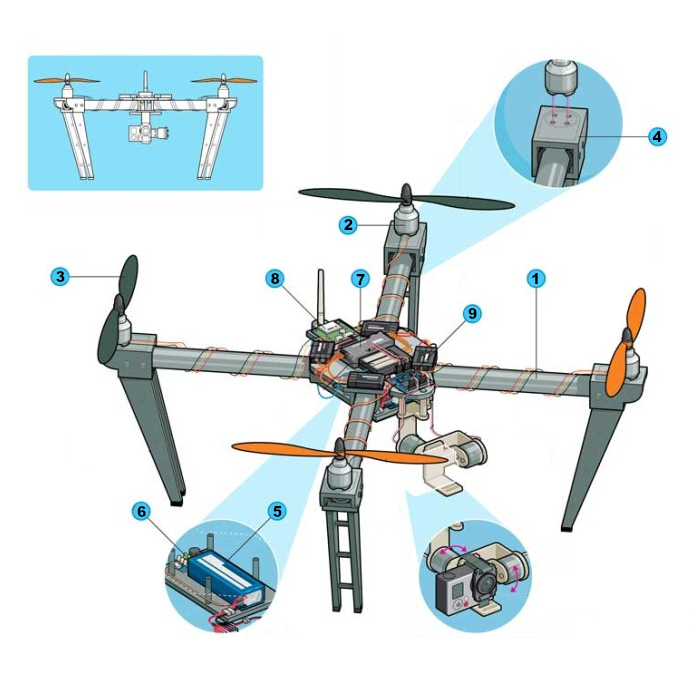
\includegraphics[width=0.5\textwidth]{soa/drone_hw_components}
    \caption[Drone hardware components]{The main hardware components of a drone are: 1. drone's frame, 2. motors, 3. propellers, 4. motor mount, 5. battery, 6. power distribution unit, 7. computing and memory unit, 8. communication unit, 9. sensors unit }
    \label{fig:drone_hw_components}
\end{SCfigure}

The software that runs on the drone, also known as the autopilot software, is usually composed of four main components: the communication unit, the sensing unit, the core control loop unit, and the low-level control unit. 
In Figure~\ref{fig:drone_sw_components}, we can see how the software components cooperate together to achieve a controllable and stable flight.
The communication unit receives and decodes commands from the off-board system; the signal is then transformed into power set-points from the core unit (control loop) with the help of sensor information. 
The sensing unit gathers information from the environment using sensors, translate 
sensor readings into readable values, then send this information to the core unit and to the communication unit to send back telemetry data to off-board systems.

\sidecaptionvpos{figure}{c}
\begin{SCfigure}[\sidecaptionrelwidth][tb]
    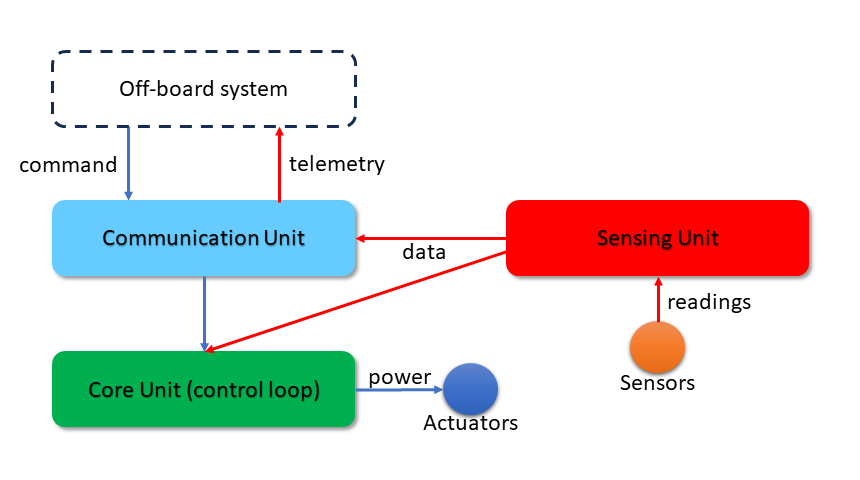
\includegraphics[width=0.7\textwidth]{soa/drone_sw_components.png}
    \caption[Drone software components]{
        The main software components of a drone are: 
        the \textit{sensing unit}, the \textit{communication unit} and the \textit{core unit (control loop)}.
    }\label{fig:drone_sw_components}
\end{SCfigure}

The current landscape of on-board drone solutions ranges from commercial off-the-shelf (COTS) to entirely custom solutions.
Commercial producers of drones like Parrot~\cite{parrot}, DJI~\cite{dij}, and 3DR~\cite{3DR} usually sell COTS solutions where all the hardware resources are supplied
with the software needed to run the drone.
Depending on the application, these bundled solutions may not be enough; if this is the case, 
the developer then needs to manually select each hardware component, control the compatibility with each other, 
and then select (or develop) the software that allows the drone to fly.

Some producer sell also intermediate solutions~\cite{pixhawk, px4, cube, navio2} between COTS and the completely custom one.
These solutions are composed of a microcontroller with usually the basic sensors that compose the 
Inertial Measurement Unit (IMU) and the autopilot software. 
These solutions are then extensible with other custom hardware; they provide programming tools to program the 
behavior of the drone during the flight.

%  TODO: reference chapter tools (section bitcraze) 
Regarding our setup, the on-board system that we used is a nano drone named Crazyflie 2.1, produced by Bitcraze; 
it is a COTS solution but with a lot of space for customization for both hardware and software components.

Off-board the drone, the environment is strongly related to the application scenario, and, in particular, it depends on the level of 
autonomy request for the drone, the flight area dimension, and the complexity of the operation.

Despite the heterogeneity of off-board systems, we can consistently identify two main components in most scenarios: a control unit and a communication unit. 
In most common situations, control and communication units are hosted on a single device.
Example of these devices are remote controls (Figure~\ref{fig:ground_station_controller}), smartphones (Figure~\ref{fig:ground_station_controller})
or a computer that acts as base (ground) station (Figure~\ref{fig:ground_base_station}).
When the scenario is more complex and the fight area is very broad, 
we can have a distributed ground network of control and communication units (Figure~\ref{fig:ground_station_distributed}).
Additionally, in combination with a distributed ground network, a sensor network can also be deployed to gather more information about the drone in its environment (Figure~\ref{fig:ground_station_distributed_with_sensor}). 
For example, the sensor network can be composed of sensors that collect atmospheric data, allowing for a better knowledge of the environment in which the drone is deployed. 

\begin{figure}[tb]
    \centering
    \subfloat[Remote control\label{fig:ground_station_controller}]{
        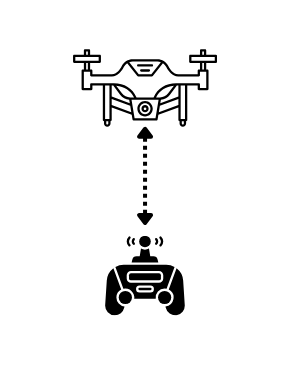
\includegraphics[width=0.25\textwidth]{soa/ground_station_controller}
    }
    \quad
    \subfloat[Smartphone\label{fig:ground_station_smartphone}]{
        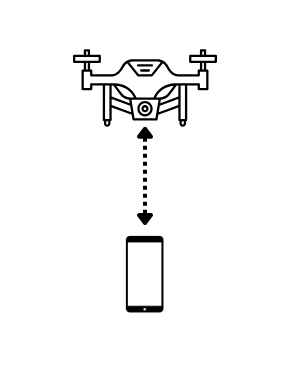
\includegraphics[width=0.25\textwidth]{soa/ground_station_smartphone}
    }
    \quad
    \subfloat[Base Station\label{fig:ground_base_station}]{
        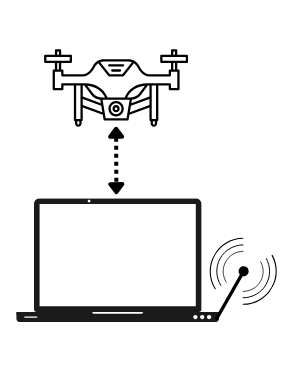
\includegraphics[width=0.25\textwidth]{soa/ground_base_station}
    }
    \quad
    \subfloat[Distributed ground network\label{fig:ground_station_distributed}]{
        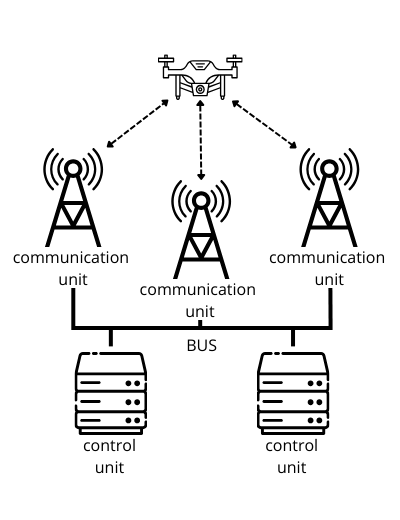
\includegraphics[width=0.35\textwidth]{soa/ground_station_distributed}
    }
    \quad
    \subfloat[Distributed ground network and sensor network\label{fig:ground_station_distributed_with_sensor}]{
        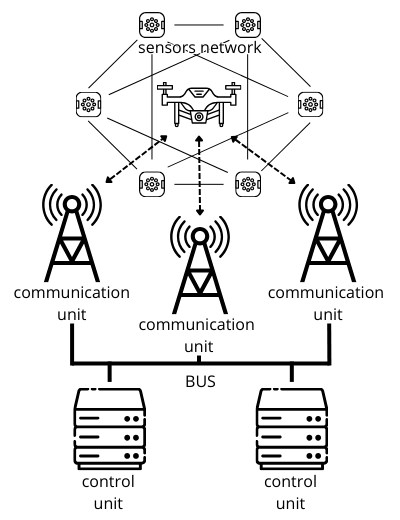
\includegraphics[width=0.35\textwidth]{soa/ground_station_distributed_with_sensor}
    }
    \caption[Off-board ecosystem]{Off-board ecosystem}\label{fig:off_board_ecosystem}
\end{figure}

Communication technology and infrastructure are critical topics that can introduce potential issues 
in the off-board environment when it is inadequate for the application scenario.
In particular, depending on the flight area's dimension, location, and topography, appropriate technology and communication infrastructure must be deployed to have a properly working drone.

As highlighted in Figure~\ref{fig:off_board_ecosystem}, the communication infrastructure can be single or distributed.
The former is more straightforward to implement and deploy but can be not enough when the flight area is too broad or the topography is irregular; 
the latter is much more complex but allows for covering all the possible application scenarios.

The most commonly used communication technology in the drone's field are Wi-Fi, radio, Bluetooth, and cellular network~\cite{pantelimon2019surveyCommunication}. 
Table~\ref{table:communication_technologies} summarizes the most common communication technologies and their characteristics.
Even if the research frontier for drone communication is mainly focused on cellular, in particular the 5G network~\cite{sharma2020communication},
none of the technologies prevails, but the choice depends on the application scenario. 
Cellular

can be a great solution around highly populated areas, while another technology must be considered in rural locations.


\begin{table}[tb]
    \centering
        \begin{tabular}{|c|c|c|c|c|}
        \hline
        \rowcolor{bluepoli!40}
        \textbf{Technology} & \textbf{Range} & \textbf{Weight} & \textbf{Complexity} & \textbf{Cost} \\
        \hline \hline
        Wi-Fi & MED [100m] & MED & HIGH & MED \\
        \hline
        Radio & SHORT-LONG [10-1000m] & LOW & LOW & LOW \\
        \hline
        Bluetooth & SHORT-MED [<25m] & LOW & MED & LOW \\
        \hline
        Cellular & LONG [8000m] & LOW & HIGH & MED \\
        \hline
        \end{tabular}
        \\[10pt]
        \caption[Communication technologies]{Communication technologies used in drone applications~\cite{pantelimon2019surveyCommunication}}\label{table:communication_technologies}
    \end{table}

The software that runs off-board is usually apt to coordinate all the resources of the environment to finally achieve and 
complete the task needed for the application. When using COTS or intermediate solutions, the vendors usually provide the 
hardware and software that compose the off-board ecosystem.

Figure~\ref{fig:easyfly_offboard_ecosystem} shows the off-board environment used in this work. 
It consists of a single base station with a USB dongle radio operating in a 2.4GHz band using a custom communication protocol named CRTP (see Section~\ref{subsec:crazyradio}). 
In substitution of a sensor network, we have an external positioning system (Lighthouse positioning system) composed of two base stations that beam the flight space with infrared, enabling the drone to measure its position by knowing the direction of infrared rays (see Section~\ref{subsec:lighthouse_hardware}).

\begin{wrapfigure}{H}{0.3\textwidth}
    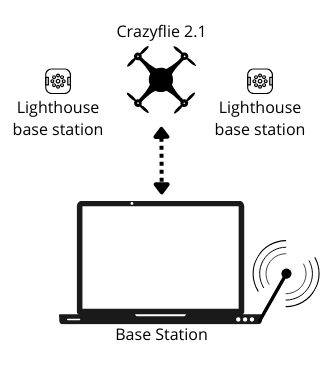
\includegraphics[width=0.3\textwidth]{soa/easyfly_offboard_ecosystem}
    \caption{EasyFly off-board ecosystem.}\label{fig:easyfly_offboard_ecosystem}
\end{wrapfigure}

A widespread problem encountered while dealing with drones is the testing phase of the application in a real environment. 
As in any other programming environment, drone programming is not immune to code bugs or hardware problems. 
Unfortunately, when an error arises, the drone will usually crash; in some unfortunate cases, some parts will break and need to be replaced. 
Therefore, testing drone applications is a very expensive task both in terms of economic resources and in terms of time. 

To overcome this limitation, the main drone producers have developed and distributed a simulation environment that allows 
testing the software before going into a real scenario. 
A simulation environment allows running the code written for the planned mission in a graphical simulation that shows the drone performing the tasks. 
Modern simulation environment~\cite{sphinx, DIJflightSimulator} usually takes into consideration atmospheric phenomena like pressure and wind to make the simulation 
closer to the real deployment environment.

In our work, we built our custom simulation tool, allowing us for a better evaluation of the work itself and, moreover, allowing  
users of our programming environment to have all the benefits of using a simulation environment (see Section~\ref{subsec:simulation_environment}).

\subsection{Swarm Programming}\label{subsec:swarm_programming}
In modern drone applications, where the tasks to achieve are complex, and the application has to be reliable, a common approach is 
to deploy multiple drones to complete the requested task collectively. This approach is completely different from single 
drone programming; in fact, swarm programming introduces new challenges and a different approach to achieving the tasks of the application.

Swarm programming is a branch of the more general swarm engineering which tries to take advantage of using multiple resources to 
achieve the application goal with better performance.

Swarm robotics and, more in general, swarm engineering is an emerging discipline that aims at defining systematic 
and well-founded procedures for modeling, designing, realizing, verifying, validating, operating, and maintaining 
a swarm robotics system. Taking inspiration from the self-organized behaviors of social animals, it makes use of simple 
rules and local interactions to design robust, scalable, and flexible collective behaviors for the coordination of large numbers of robots.
The inspiration that swarm robotics takes from the observation of social animals (ants, bees, birds, fish, …) is that starting from simple individuals,
they can become successful when they gather in groups, exhibiting a sort of swarm intelligence~\cite{bonabeau1999swarm}.

In particular, the behavior of social animal groups appears robust, scalable, and flexible. 
Robustness is the ability to cope with the loss of individuals. 
In social animals, robustness is promoted by redundancy and the absence of a leader. 
Scalability is the ability to perform well with different group sizes. 
The introduction or removal of individuals does not result in a drastic change in the performance of a swarm. 
In social animals, scalability is promoted by local sensing and communication. 
Flexibility is the ability to cope with a broad spectrum of different environments and tasks. 
In social animals, flexibility is promoted by redundancy, simplicity of the behaviors, and mechanisms such as task allocation.

Two great examples in the current literature of swarm engineering are Proto~\cite{bachrach2010proto} and Meld~\cite{ashley2007meld}. 
The former is a spatial computing language that allows programming swarms of robots starting from a mathematical model called amorphous medium.
The latter is a declarative programming language that uses logic programming to enable swarm programming.
Both languages directly take the swarm programming from the point of view of aggregate behaviors, i.e., their approach is to program the entire
swarm behavior instead of programming every single component separately.

When swarm robotics is applied in the field of drones, given the high dynamism in the movements of this type of robot, 
the swarm management and control is much more complex with respect to the single drone, 
but the capability of the swarm may increase the application's performance.

In the first place, the swarm, compared to the single drone, can provide a higher availability.
A single drone has a limited flight time, so its batteries need to be recharged or replaced. A swarm instead can dynamically 
deploy and retire drones to be always active on the field. In addition, a swarm can also scale when the request 
increases, e.g., a phenomenon to sense has a peak of occurrence~\cite{dantu2011karma}. 
In the same situation, a single drone application can miss the peak of the phenomena because, for example, it can be stuck at the charging station.

With swarms, the goal of the application is usually defined as a swarm goal.
Swarm goals are high-level goals whose achievement is independent of the success or the failure of the single task of a swarm component.
The separation between application (swarm) goals and drone tasks allows the application to be scalable and fault-tolerant.
Of course, the advantages of the swarm with respect to the single drone hide inside a huge complexity.
As the number of components of the swarm increases, the complexity of managing all of them increases, 
introducing a consistent overhead that can affect the application's performance.
As in any other engineering problem, we must select and identify the most suitable swarm size for the application to realize.

Depending on the application domain, we can adopt different strategies for coordinating the resources available.
We can identify three main programming models that can be applied to swarm programming in the field of drones: drone-level programming, swarm programming, and team-level programming.

Drone-level programming is the most straightforward approach; it expects to develop a single application for each component of the swarm, 
taking into account all the possible interactions between them. 
This finest grain method allows an entirely independent, customizable, and deterministic single-drone behavior. 
Since the application has a swarm goal that is not directly related to the single drone's task, 
with this method, it is usually tricky to use all the swarm resources efficiently to reach the general goal. 
Moreover, it has been proven~\cite{mottola2014team, dantu2011karma} that this method is indeed the most complex of the three in terms of programming effort.

Swarm programming~\cite{quigley2009ros}, on the other hand, allows writing a single set of rules that are common for all drones, and then every single drone 
executes that instruction in its local state. The swarm programming model explicitly forbids a shared or global state.
This programming model is easier to use and to set up and scale up with multiple drones, but it is challenging to represent tasks that require explicit drone coordination.

Team level programming~\cite{mottola2014team} is a programming model in between swarm and drone level programming, 
in which users express sophisticated collaborative sensing tasks without resorting to individual addressing 
and without exposure to the complexity of concurrent programming, parallel execution, scaling, and failure recovery.
The model can be viewed as a set of tasks that must be performed by a set of drones subject to particular timing and spatial constraints~\cite{mottola2014team}.

Our work does not address the complexity of swarm programming, although our programming environment, EasyFly, allows for the deployment of multiple drones (see Chapter~\ref{ch:conclusions}).